\documentclass[12pt,twoside,openright,a4paper,final]{book}
\linespread{1.25}

\usepackage[margin=1in]{geometry}
\usepackage{subfig}
\usepackage{graphicx}
\usepackage[space]{grffile}
\usepackage{latexsym}
\usepackage{textcomp}
\usepackage{longtable}
\usepackage{multirow,booktabs}
\usepackage{amsfonts,amsmath,amssymb}
\usepackage[hyphens]{url}
\usepackage[numbers]{natbib}
\usepackage{hyperref}
\hypersetup{colorlinks=false,pdfborder={0 0 0}}
% You can conditionalize code for latexml or normal latex using this.
\newif\iflatexml\latexmlfalse
\usepackage[utf8]{inputenc}
\usepackage[ngerman,english]{babel}
\usepackage{mcode} % Maltab code
\usepackage{authblk} % Multiple authors
\usepackage[section]{placeins}
\usepackage{rotating}
\usepackage{units}
\usepackage{siunitx}
\usepackage{fancyhdr}
\setlength{\headheight}{14.5pt} % Fix warning
\usepackage{enumitem}
\usepackage{lastpage}
\usepackage{epstopdf}
\usepackage{siunitx}
\usepackage{tocstyle}

%START added packages used by Orbiter (Johannes Linde)
\usepackage{verbatim}
\usepackage{bigstrut}
\usepackage{tablefootnote}
\usepackage{placeins}
\usepackage{pdfpages}
%\usepackage[disable]{todonotes}
\usepackage{todonotes}
\usepackage{multicol}
\setlength{\columnsep}{0cm}
%END added packages used by Orbiter (Johannes Linde)

\setlist[enumerate]{noitemsep}
\setlist[itemize]{noitemsep}


\makeatletter
\AtBeginDocument{%
  \expandafter\renewcommand\expandafter\subsection\expandafter{%
    \expandafter\@fb@secFB\subsection
  }%
}
\makeatother

%\newcommand{\mycourse}[0]{30320 Spacecraft Instrumentation Systems}

\pagestyle{fancy}
\fancyhf{}
\renewcommand{\chaptermark}[1]{\markboth{
	\if@mainmatter
		\ifnum0\thechapter<1
			\MakeUppercase{#1}
		\else
			\thechapter.\; \MakeUppercase{#1}
		\fi
	\else
		\thechapter.\; \MakeUppercase{#1}
	\fi
}{}}
%\fancyhead[LE,RO]{\thepage}
%\fancyfoot{}
%\fancyfoot[L]{\begin{footnotesize}{\textsc{Page \thepage{ }of \pageref*{LastPage}}}\end{footnotesize}}
%\fancyfoot[R]{\begin{footnotesize}{\textsc{\mycourse}}\end{footnotesize}}
\fancyhead[LE,RO]{\thepage}
\fancyhead[RE]{\slshape \rightmark}
\fancyhead[LO]{\slshape \leftmark}

\providecommand{\e}[1]{\ensuremath{\times 10^{#1}}}

\newcommand{\HRule}{\rule{\linewidth}{0.5mm}} % \HRule for special horizontal line

\makeatletter
\newcommand{\addauthorbelowheading}[1]{%
	{\parindent0pt\vspace*{-10pt}%
  	\linespread{1.1}\small\scshape#1%
  	\par\nobreak\vspace*{10pt}}%
  	\@afterheading%
}
\makeatother

\newcommand\autchapter[2]{%
	\chapter[#1{\normalfont\tiny\itshape ~- #2}]{#1%
  		\chaptermark{#1}}%
	\chaptermark{#1}%
	\addauthorbelowheading{#2}%
}

% Use theses command to add section and subsection authors
\newcommand\autsection[2]{%
	\section[#1{\normalfont\tiny\itshape ~- #2}]{#1%
		\sectionmark{#1}}%
	\sectionmark{#1}%
	\addauthorbelowheading{#2}%
}

\newcommand\autsubsection[2]{%
	\subsection[#1{\normalfont\tiny\itshape ~- #2}]{#1%
  		\subsectionmark{#1}}%
	\subsectionmark{#1}%
	\addauthorbelowheading{#2}%
}

% DTU frieze
\usepackage{eso-pic}
\newcommand{\frieze}{%
    \AddToShipoutPicture*{
        \put(-5,-30){
            \parbox[b][\paperheight]{\paperwidth}{%
                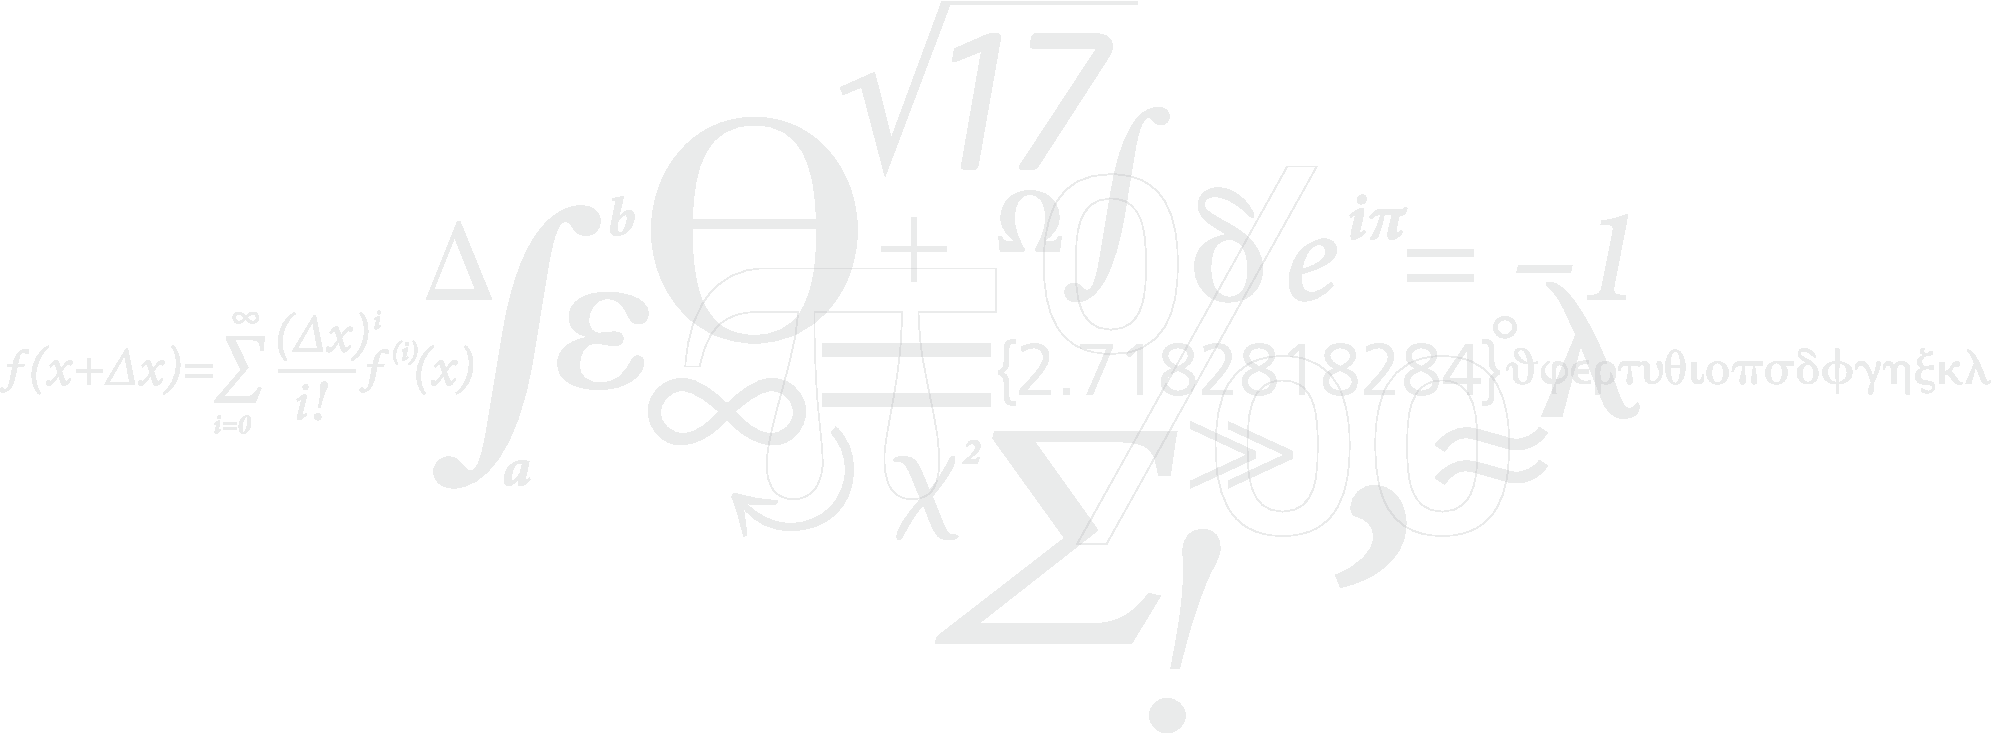
\includegraphics[trim=130mm 0 0 0,width=0.9\textwidth]{figures/DTU-frise-SH-15}
                \vspace*{2.5cm}
            }
        }
    }
}

\newcommand{\logoElektro}{%
    \AddToShipoutPicture*{
        \put(20,-50){
            \parbox[b][\paperheight]{\paperwidth}{%
                
\includegraphics[width=0.6\textwidth]{figures/tex_dtu_space_a_uk}
                \vspace*{2.5cm}
            }
        }
    }
}

\makeatletter
\newcommand{\prefrontmatter}{
	\thispagestyle{empty}
	\begin{center}
	\vspace*{1cm}
	\large\textsc{Technical University of Denmark}
	\HRule \\[1cm]
	\@title\\[0.7cm]
	\HRule \\%[1cm]
	\begin{center}
       	
\includegraphics[width=0.2\textwidth]{figures/tex_dtu_logo}
	\end{center}
%	\vspace{0.7cm}
	\normalsize \@author
%	\vfill
	\vspace{1.5cm}\\
	{\normalfont \large \@date}
	\end{center}
	\frieze
	\logoElektro
    \newpage % Back of front page
    \thispagestyle{empty}
	\frieze % Added watermark
	\hspace*{-1cm}
	\parbox[b][\paperheight]{\paperwidth}{%
		{\sf Technical University of Denmark}\\
		{\sf DTU Space}\\
		{\sf National Space Institute}\\
		{\sf Elektrovej, building 327-328}\\
		{\sf 2800 Kongens Lyngby, Denmark}
	    \vspace*{10cm}
	}
}
\makeatother

\date{Kongens Lyngby, June 2016}

\title{\huge{Spacecraft Instrumentation Systems \\ Europa Life Finder Mission}}

\author{Jean-Paul Breuer}
\author{Aaron Gornott}
\author{Yannis Nissopoulos}
\author{Fruzsina Bacsó}
\author{Ricard Lladó Grove}
\author{Gustavo Feijóo Carrillo}
\author{Johannes Linde}
\author{Maja Tomicic}
\author{Agge Winther}
\author{Paul Connetable}
\author{Rasmus Lundby Pedersen}
\author{Bhaaeddin Alhomsi}
\author{Ifikratis Kamenidis}
\author{Paschalis Dalampiras}
\author{Lukas Christensen}
\author{Morten Lykke Hilligsøe}
\author{Søren Jeppesen}
\author{Sebastian Helvig Christensen}
\author{Kristian Sloth Lauszus}

\affil{National Space Institute, Technical University of Denmark}
\renewcommand\Affilfont{\itshape\small}
\setcounter{Maxaffil}{0}
